\item  No instante $\theta=45^{\circ}$, o membro $DC$ tem uma velocidade angular $\omega_{DC}=\SI{4}{\radian/\second}$ e uma aceleração angular $\alpha_{DC}=\SI{2}{\radian/\second^{2}}$. Determine a velocidade angular e a aceleração angular da barra $AB$ nesse instante. O anel em $C$ está conectado por pino a $DC$ e desliza livremente ao longo de $AB$.

\import{../answers/}{answer-14}

\begin{flushright}
	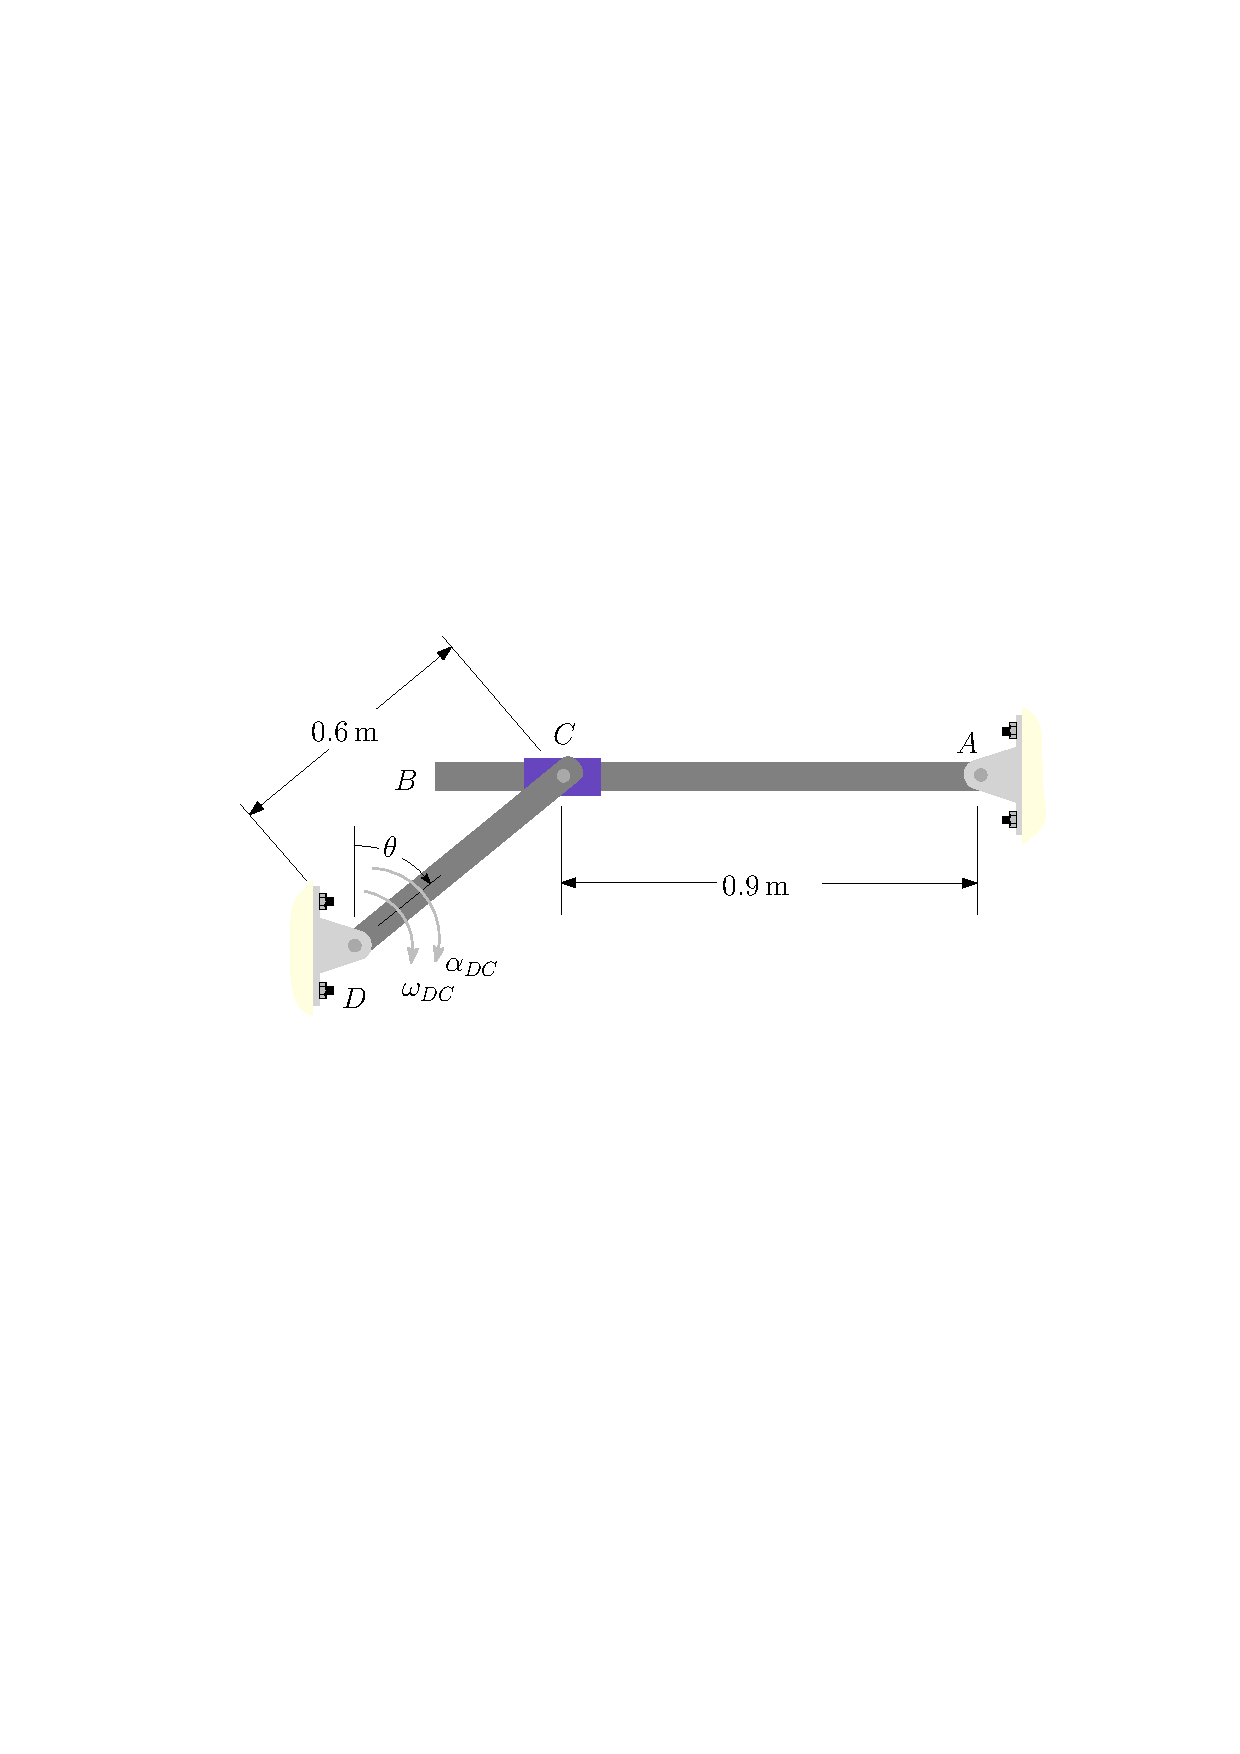
\includegraphics[scale=1]{images/draw_12}
\end{flushright}